\chapter{Programming geoalgorithms}\label{ProgrammingGeoalgorithms}
 

 \section{Introduction. Initial settings}

This chapter introduces the fundamental ideas needed to implement a new geoalgorithm based on SEXTANTE. Using the SEXTANTE framework to create a new geoalgorithm will allow it to be used in any of the components of SEXTANTE (toolbox, graphical modeler, etc.), and in any of the applications that integrate SEXTANTE, without any modification at all.

The first thing to do to create your own SEXTANTE geoalgorithm is to create a project. Let's create a new project named \emph{MyAlgorithms}:

Since it will depend on SEXTANTE base classes, the next thing to do is to add the SEXTANTE jar files to the list of referenced libraries. Create a folder named ``lib'' in your project and add the following files:

\begin{itemize}
\item \texttt{sextante.jar}: The SEXTANTE core classes
\item \texttt{jts-1.12.jar}: Java Topology Suite, used for handling geometries
\item \texttt{kxml2.jar}
\item \texttt{jfreechart-1.0.1.jar}: JFreeChart library, used for generating charts as output of geoalgorithms
\item \texttt{jcommons-1.0.0.jar}: Base elements for the JFreeChart library.
\end{itemize}
 
 Add this files to the build path of the project.
 
 Now create a new package to put your first geoalgorithm on it. You can use any name you want, but here we will stick to the naming conventions used in the SEXTANTE library.

Create a package and name it \texttt{es.unex.sextante.multiplyRaster}. Usually, a new package is created for each single algorithm, which will contain all the necessary files to describe and implement that algorithm. As we will see, this is usually done using a single file.
 
 Let's add the file that will contain our algorithm. The class name will be used to generate the command--line name of the algorithm, and the file containing the algorithm has to end with the suffix ``Algorithm''. For this reason, you should try to give your class a descriptive name, so when using it from the command--line it is easy to understand what it does. In this case we will name it \texttt{MultiplyRasterAlgorithm}, so later we could call it from the command line using the command \texttt{multiplyraster}.

 You should have something like this:

\begin{center}
 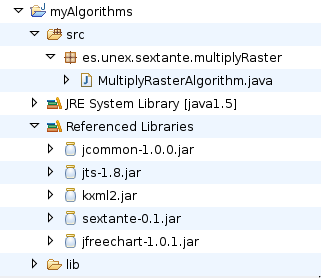
\includegraphics[width=.5\textwidth]{myalgs_project.png} 
\end{center}

 \section{The \texttt{GeoAlgorithm} class. Creating a geoalgorithm}
 
 All geoalgorithms must extend the \texttt{GeoAlgorithm} class, which provides the foundation for all the operations needed to perform any kind of geospatial analysis.
 
To implement your geoalgorithm you just have to implement two methods:

 \begin{itemize}
\item \texttt{defineCharacteristics()}
\item \texttt{processAlgorithm()}
\end{itemize}
 
 
 The first of them should be used to define the characteristics of the algorithm. These characteristics will be used for such things as defining the user interface or selecting the correct way of linking it with other algorithms within a model. Basically, this method should give an answer to the following questions:
 
 
\begin{itemize}
	\item Which inputs are needed to run the algorithm?
	\item Which outputs will this algorithm generate?
	\item Basic characteristics of the algorithm (name, group it belongs to, etc.)
\end{itemize}

The \texttt{processAlgorithm()} method is where you have to implement the algorithm itself, adding all the calculations and processes that constitute it.

We are going to create a simple algorithm that takes a raster layer and a numerical value, and generates a new raster layer which is the result of multiplying the input raster layer and the value (i.e. multiplying the value of each cell in the raster layer and the numerical vale).
 
\subsection{Defining the characteristics of the algorithm}
 
 To set the characteristics of the algorithm you have to add all necessary definitions in the \texttt{defineCharacteristics()} method. This method is called upon construction of the geoalgorithm.
 
 For our first example, we will add the following code to this method:
 
  \begin{verbatim}
public void defineCharacteristics() {

  this.setName("Multiply raster");
  this.setGroup("My algorithms");
  this.setUserCanDefineOutputExtent(false);
				
  try {
    m_Parameters.addInputRasterLayer("INPUT", "Raster layer", true);
    m_Parameters.addNumericalValue("VALUE",
           "Value",
           1,
           AdditionalInfoNumericalValue.NUMERICAL_VALUE_DOUBLE);
    addOutputRasterLayer("RESULT", "Result");
  } catch (RepeatedParameterNameException e) {
    e.printStackTrace();
  }

}
\end{verbatim}
 
Let's analyze this code.
 
 The first line sets the name of the algorithm. When using the toolbox or the graphical modeler, this will be the name that will identify the algorithm. The \texttt{setGroup(String)} method is used to set the group the algorithm belongs to.
 
In case you want to, you can give the user the option to select the characteristics of the output layers (extent for vector layers or extent and cellsize for raster ones). This will cause SEXTANTE to add anew tab in the algorithm dialog. The information entered by the user in this tab can later be retrieved and used as the analysis region, restricting the area anayzed by the algorithm or the extent of the output layer it generates. In our case, we are going to generate a new raster layer with exactly the same characteristics as the input layer, so there is no need to let the user select a different extent or cellsize. 
 
 Whenever you do not want the user to be able to select output layer characteristics, you can add the following line
 
 \begin{verbatim}
 setGeneratesUserDefinedOutput(false);
 \end{verbatim}
 
 \noindent to indicate that SEXTANTE should not show the output tab, even though the algorithm generates new layers.
 
 We will see how to deal with output extents (whether they have been set by the user or not) in a different section, so now you do not really have to worry about that.
 
To tell SEXTANTE that our algorithm needs a raster layer and a numerical value, we will use the \texttt{m\_Parameters} field of the \texttt{GeoAlgorithm} class. This field is an object of class \texttt{ParametersSet}, which is basically a container of objects of class \emph{Parameters}. This parameters define the inputs needed by the algorithm, and describe the particular characteristics of each one them.

the \texttt{ParametersSet} class has several method to easily add parameters to it. Here is a list of the main ones, along with the kind of parameters that they add:

\begin{itemize}
	\item To add a raster layer,
	\begin{verbatim}
public void addInputRasterLayer(String sName,
	                              String sDescription,
                                boolean bIsMandatory)}                                                    
\end{verbatim}
The two first arguments appear on every method that we are going to see in this section. The first one is the name used to identify the parameter, and it has to be unique. The second one is the description (human--readable) of the algorithm. This will be the one used to name the algorithm in the parameters window.

As an example, here is the line that can be found in the \emph{Slope} algorithm to indicate that a raster layer (a DEM) is needed to run it:

\begin{verbatim}
m_Parameters.addInputRasterLayer(DEM, Sextante.getText("DEM"), true);
\end{verbatim}

\texttt{DEM} is defined as a String constant within that same class.

\begin{verbatim}
	public static final String DEM = "DEM";
\end{verbatim}

This is a good practice, since it makes it easier to call algorithms from other classes. For this reason, you should always create public constants when defining parameter names, as this will make your algorithms easier to reuse.

The \texttt{Sextante.getText()} method is a static method used to support internationalization. We will see how to use that in a different section in this same chapter.

\item To add a vector Layer,
\begin{verbatim}
public void addInputVectorLayer(String sName,
                                String sDescription,
                                int iShapeType, 
                                boolean bIsMandatory)
\end{verbatim}

This method is similar to the one used to add raster layers, except for an additional parameter that indicates the type of vector layer that is needed. Values for this parameter can be any of the following constants. Names are pretty self--explanatory.

\begin{itemize}
	\item \texttt{AdditionalInfoVectorLayer.SHAPE\_TYPE\_POINT}:  
	\item \texttt{AdditionalInfoVectorLayer.SHAPE\_TYPE\_LINE}: 
	\item \texttt{AdditionalInfoVectorLayer.SHAPE\_TYPE\_POLYGON}: 
	\item \texttt{AdditionalInfoVectorLayer.SHAPE\_TYPE\_ANY}: 
\end{itemize}



We find an example of this method in those algorithms that perform some kind of interpolation, which take a points layer as input

\begin{verbatim}
m_Parameters.addInputVectorLayer(LAYER, Sextante.getText("Points_Layer"),
                  AdditionalInfoVectorLayer.SHAPE_TYPE_POINT,
                  true);
\end{verbatim}

\item To add a table

\begin{verbatim}
public void addInputTable(String sName,
                          String sDescription,
                          boolean bIsMandatory)
\end{verbatim}

\item To add a numerical value

There are two methods that can be used. The first one will not restrict the values that the user can enter.

\begin{verbatim}
public void addNumericalValue(String sName,
                              String sDescription,
                              double dDefaultValue,
                              int iType)
\end{verbatim}

The last argument is used to indicate whether the value is a floating point or an integer one. Use one of the following constants:

\begin{itemize}
	\item \texttt{AdditionalInfoNumericalValue.NUMERICAL\_VALUE\_INTEGER}: 
	\item \texttt{AdditionalInfoNumericalValue.NUMERICAL\_VALUE\_DOUBLE}: 
\end{itemize}

For our first algorithm, the value to be used to multiply the input raster layer can take any value. We will set a default value of 1. The line to add to the \texttt{defineCharacteristics()} will be the next one.

\begin{verbatim}
m_Parameters.addNumericalValue("VALUE",
           "Value",
            1,
            AdditionalInfoNumericalValue.NUMERICAL_VALUE_DOUBLE);
\end{verbatim}

In some cases, however, it is necessary to define a range of valid values. If so, the next method should be used instead of the previous one.

\begin{verbatim}
public void addNumericalValue(String sName,
                              String sDescription,
                              double dDefaultValue,
                              int iType,
                              double dMinValue,
                              double dMaxValue)
\end{verbatim}

No matter what the type of the value (integer or double), minimum and maximum values are always entered as double ones.

Here is an example, from the \emph{Density} algorithm, which needs a search radius that has to be non--negative.

\begin{verbatim}
m_Parameters.addNumericalValue("DIST", Sextante.getText("Search_radius"), 
              AdditionalInfoNumericalValue.NUMERICAL_VALUE_DOUBLE,
              100, 0, Double.MAX_VALUE);
\end{verbatim}

\item To add a string

\begin{verbatim}
public void addString(String sName,
                      String sDescription,
                      String sDefaultString)
\end{verbatim}

If no default value is needed, you can pass an empty string or use the following simplified method.

\begin{verbatim}
public void addString(String sName,
                      String sDescription)
\end{verbatim}

For example, this line can be found in the \emph{Raster calculator} algorithm.
\begin{verbatim}
m_Parameters.addString(FORMULA, Sextante.getText("F�rmula"));
\end{verbatim}

\item To add a boolean parameter.

\begin{verbatim}
public void addBoolean(String sName,
                       String sDescription)
\end{verbatim}

\item To add a selection.

It is common to request the user to select from a list of valid values. To do so, use the following method:

\begin{verbatim}
public void addSelection(String sName,
                         String sDescription,
                         String[] sValues)
\end{verbatim}	

\noindent where \texttt{sValues} is an array of strings with the names of all the possible options.

For example, if you would like the user to select a method from a list of three available ones.
\begin{verbatim}
String[] sMethod = {"Method 1", "Method 2", "Method 3"};
m_Parameters.addSelection("METHOD", "Method", sMethod);
\end{verbatim}  
                 
\item to add an editable table

Although we have already seen how to add a table to the parameters list, there is another kind of tables that SEXTANTE can use as input. In some cases you might require a small table such as a look--up table or a $3\times 3$ table to be used as a kernel for convolution operation. In this case, SEXTANTE will show the table and the user will define its values when executing the algorithm, instead of using an existing table.

The following method is used to incorporate this kind of parameter to the algorithm.

\begin{verbatim}
public void addFixedTable(String sName,
                          String sDescription,
                          String[] sColumnNames,
                          int iRows,
                          boolean bIsNumberOfRowsFixed)
\end{verbatim}

The number of columns is fixed, and is defined by the length of the \texttt{sColumnNames} argument. The number of rows is defined using the \texttt{iRows} argument, but it does not have to be fixed. In some cases, it is interesting to let the user add new rows or remove them according to his needs. In other cases (like, for instance, when defining a $3\times 3$ kernel), the initial number of rows should not be modified. To set how SEXTANTE should behave, the last argument of the method is used.

In the aforementioned convolution algorithm, we find the following line:

\begin{verbatim}
String sColumnNames[] =  {"1", "2", "3"};
m_Parameters.addFixedTable(KERNEL, Sextante.getText("Kernel"), 
                           sColumnNames, 3, true);
\end{verbatim}

\item To add a point.

\begin{verbatim}
public void addPoint(String sName,
                     String sDescription)
\end{verbatim}

\item To add a multiple input

When you do not need a single layer, but a list of them, the \emph{addInputRasterLayer()} method that we already know is not enough. The \texttt{ParametersSet} class contains a method to add a multiple input that can be an array of vector layers, raster layers or tables.

\begin{verbatim}
public void addMultipleInput(String sName,
                             String sDescription,
                             int iDataType,
                             boolean bIsMandatory)
\end{verbatim}

Like single inputs, multiple inputs can be mandatory or optional.

Using the \emph{iDataType} argument, the type of input can be set, using one of the following constants:

\begin{itemize}
	\item \texttt{AdditionalInfoMultipleInput.DATA\_TYPE\_RASTER} 
	\item \texttt{AdditionalInfoMultipleInput.DATA\_TYPE\_VECTOR\_POINT}
	\item \texttt{AdditionalInfoMultipleInput.DATA\_TYPE\_VECTOR\_LINE} 
	\item \texttt{AdditionalInfoMultipleInput.DATA\_TYPE\_VECTOR\_POLYGON} 
	\item \texttt{AdditionalInfoMultipleInput.DATA\_TYPE\_VECTOR\_ANY} 	
	\item \texttt{AdditionalInfoMultipleInput.DATA\_TYPE\_VECTOR\_TABLE} 
	\item \texttt{AdditionalInfoMultipleInput.DATA\_TYPE\_BAND}
\end{itemize}

An example of this can be found in the \emph{Merge raster layers} algorithm.

\begin{verbatim}
m_Parameters.addMultipleInput(INPUT, Sextante.getText("Layers_to_merge"), 
                      AdditionalInfoMultipleInput.DATA_TYPE_RASTER);
\end{verbatim}

\end{itemize}

Apart from these ones, two other parameters can be added, which are not independent but depend on some other parameter previously introduced. 

\begin{enumerate}
	\item To add a field from a vector layer or a table.
	
The same method is used in both cases, since the attributes table of a layer is handled just as independent table.
	
\begin{verbatim}
public void addTableField(String sName,
                          String sDescription,
                          String sParentParameterName)
\end{verbatim}	

The key argument here is the last one, which indicates the name of the parameter that acts as the parent parameter of this one. It has to be a vector layer or table, and its name (the value passed to the \texttt{sName} argument when adding that layer) has to be used to select it.

Here is an example, where a table parameter is defined and then two parameters representing two fields from that table are added.

\begin{verbatim}
m_Parameters.addInputTable("TABLE", "Table", true); 
m_Parameters.addTableField("XFIELD", "X coordinate", "TABLE");
m_Parameters.addTableField("YFIELD", "Y coordinate", "TABLE");
\end{verbatim}

\item To add a band from a raster layer.

The syntax of the method is identical to the previous one.

\begin{verbatim}
public void addBand(String sName,
                    String sDescription,
                    String sParentParameterName)
\end{verbatim}		

And here is an example from the \emph{NDVI} algorithm			

\begin{verbatim}
m_Parameters.addInputRasterLayer("LAYERRED", "Red layer", true);
m_Parameters.addBand("BANDRED", "Red band", "LAYERRED");
\end{verbatim}

\end{enumerate}

All this should be enough to define the requirements of the algorithm. The outputs of the algorithm also have to be defined, in order to have enough information to use it in the graphical modeler. If output results are not defined, we will be able to execute the algorithm, but the grammar of the process will not be complete, and other operations will not be available.

Adding outputs is similar to adding input parameters. There are a few convenience methods in the \texttt{GeoAlgorithm} class that can be used for this purpose. These are used to add the six types of outputs supported by SEXTANTE: raster layers, vector layers, tables, numerical values, graphs and texts.

\begin{itemize}
	\item To add a raster layer
	
	\begin{verbatim}
protected void addOutputRasterLayer(String sName, 
                                    String sDescription,
                                    int iBands) {
			
	\end{verbatim}
	
	Just like input parameters, outputs need a name and a description, the first one being unique and used to identify them (we will later see why this is important) and the second one to show to the user in the corresponding parameters window.
	
	In the case of raster layers, the number of bands expected for the output layer has to be entered using the \texttt{iBands} argument. In case this cannot be known in advance, the \texttt{OutputRasterLayer} provides a constant to indicate it:
	
	\begin{verbatim}
	OutputRasterLayer.NUMBER_OF_BANDS_UNDEFINED
	\end{verbatim}
	
For the most usual case of adding a single--band raster layer, a simplified method exists.
	
		\begin{verbatim}
protected void addOutputRasterLayer(String sName, 
                                    String sDescription,
                                    int iBands) {
			
	\end{verbatim}
	
	\item To add a vector layer

	\begin{verbatim}
protected void addOutputVectorLayer(String sName, 
                                   String sDescription,
                                   int iType) {
	\end{verbatim}
	
	In this case, instead of setting the number of bands, the type of vector layer that is expected has to be entered. The following constants can be used for the corresponding argument.
	
	\begin{verbatim}
OutputVectorLayer.SHAPE_TYPE_POLYGON
OutputVectorLayer.SHAPE_TYPE_POINT
OutputVectorLayer.SHAPE_TYPE_LINE
OutputVectorLayer.SHAPE_TYPE_UNDEFINED
	\end{verbatim}
	
	The last one should be used when the type of layer cannot be known in advance and is selected at run time.
	
	\item To add a text output.

	\begin{verbatim}
protected void addOutputText(String sName, 
                                   String sDescription) {
	\end{verbatim}
	
	
	\item To add a text output.

	\begin{verbatim}
protected void addOutputChart(String sName, 
                                   String sDescription) {                                                                      
	\end{verbatim}
	
	\begin{verbatim}
protected void addOutputChart(String sName, 
                                   String sDescription) {                                                                      
	\end{verbatim}	
		
	In these three last cases, no information apart from the name and the description is needed about the outputs. 
	
	Numerical values are a particular type of output. Usually these values are presented in a simple text to the user. However, you can also declare them and that will add extra information to the semantics of the algorithm. By doing this, numerical values generated by an algorithm could be used as input to any other algorithm that takes a numerical value as input, when combinign them in the graphical modeller. Other than that, numerical values themselves are not shown to the user (unless you explicitly put them into a text output).
	
\end{itemize}

\subsection{Implementing the process}

As it has been said, the algorithm itself has to be implemented in the \texttt{processAlgorithm()} method, which will be called when the algorithm is executed. Before executing the process, input parameters have to be given valid values. This is done by SEXTANTE when the user selects those values in the parameters window, or is done programmatically before executing the algorithm, as we saw in chapter \ref{UsingAlgorithms}.

Here is the code of the method, which we will discuss next.


\begin{verbatim}
public boolean processAlgorithm() {
  
  int x,y;
  int iNX, iNY;
  double dValue;
  double dConstant;		
  IRasterLayer layer ;
  
  layer = m_Parameters.getParameterValueAsRasterLayer("INPUT");
  dConstant = m_Parameters.getParameterValueAsDouble("VALUE");
    
  AnalysisExtent outputExtent = new AnalysisExtent(layer); 	
  IRasterLayer result = getNewRasterLayer("RESULT", "Result",
                              IRasterLayer.RASTER_DATA_TYPE_FLOAT,		
                              outputExtent);
			
  layer.setWindowExtent(outputExtent);
  iNX = outputExtent.getNX();
  iNY = outputExtent.getNY();
			
  for(y = 0; y < iNY && setProgress(y, iNY);; y++){		
    for(x = 0; x < iNX; x++){
      dValue = window.getCellValueAsDouble(x, y);
      result.setCellValue(x, y, dValue * dConstant);
    }
  }

  return !m_Task.isCanceled();
		
}
\end{verbatim}

There are three main task to accomplish when implementing the algorithm.

\begin{itemize}
	\item Retrieve values from input parameters. Values have to be recovered and put into variables to make them easier to use for the algorithm process.
	\item Operate with those variables. Of course, we are not going to tell you how to perform this second task, since it is up to you to implement your own algorithm. However, we will see some examples about how to use the basic interfaces for raster layers, vector layers and tables, which are the ones that you will be using to access the input data.
	\item Create output results. Outputs are the most important part of the algorithm (they are the reason to execute it!), and have to be correctly defined, so SEXTANTE can use those outputs in other algorithms and deal with them.
\end{itemize}

To retrieve parameter values, we have to use the \texttt{m\_Parameters} object once again. When we added parameters using its methods in the \texttt{defineCharacteristics()} method, new objects of class \texttt{Parameter} were added with a null value. Now they contain a value and that is the value that we have to retrieve.

The \texttt{ParametersSet} class contains several methods with a similar syntax, which should be used depending of the type of value to be retrieved. Here is a list of all the available methods.

\begin{verbatim}
public int getParameterValueAsInt(String sParameterName) 
public double getParameterValueAsDouble(String sParameterName)
public Point2D getParameterValueAsPoint(String sParameterName) 
public boolean getParameterValueAsBoolean(String sParameterName) 
public ArrayList getParameterValueAsArrayList(String sParameterName) 
public String getParameterValueAsString(String sParameterName) 
public FLyrVect getParameterValueAsVectorLayer(String sParameterName) 
public FLyrRaster getParameterValueAsRasterLayer(String sParameterName) 
public DataSource getParameterValueAsTable(String sParameterName) 
\end{verbatim}

They all take one string, which is the name of the parameter from which to retrieve the value. This is the name that was used to define the parameter when it was added to the \texttt{defineCharacteristics()} method.

For most cases, it is easy to figure out the method to use. Using a wrong method will cause a \texttt{WrongParameterTypeException}. exception to be thrown. For example, it does not make sense to get the value of a numerical parameter as a raster layer using the  \texttt{getParameterValueAsRasterLayer()} method.

If the parameter does not have a value assigned, calling any of the above methods will throw a \texttt{NullParameterValueException} exception. Layers and tables can be optional, and in this case the null value is a valid one, so it can be returned. If the parameter is mandatory, however, the exception is thrown.

The  \texttt{getParameterValueAsInt(String)} method is used not only to get the value of a numerical parameter, but also the value of a selection (returns the zero--based index of the selected element), a band (the zero--based index of the chosen band) or a table field (the zero--based index of the field).

You can always use the \texttt{getParameterValueAsObjectInt(String)} and then cast the returned object to the corresponding class. For fixed tables, added using the \texttt{addFixedTable} method, the value is returned as an object of class \texttt{FixedTableModel}, which is a class extending the Java \texttt{AbstractTableModel} class.

Here is an example:

\begin{verbatim}
FixedTableModel lut = (FixedTableModel) m_Parameters.
                       getParameterValueAsObject("LUT");
\end{verbatim}

With the above methods, we can easily understand how the raster layer and the numerical value needed for our algorithm are retrieved.

Once we have those values, it is time to create the output layer. In this case, we will generate a new raster layer and later on set the corresponding values in its cells.

To generate a new output you can create a new instance of the corresponding class (in this case it would be a \texttt{OutputRasterLayer}) and then add it to the set of output object using methods in the \texttt{OutputObjectsSet} class. We will use this approach when generating charts or texts as results, but in the case of layers or tables it is much more practical to use some of the methods provided by the \emph{GeoAlgorithm} class. This is not only easier but also safer, and it is the recommended way of doing it.

Here is a short list of the methods available for creating new layers and tables.

\begin{verbatim}
 protected IVectorLayer getNewVectorLayer(String sName, 
                                          String sDescription,
                                          int iShapeType,
                                          Class[] types, 
                                          String[] sFields);

protected IRasterLayer getNewRasterLayer(String sName,
                                         String sDescription,
                                         int iDataType,
                                         int iBands){

protected IRasterLayer getNewRasterLayer(String sName,
                                         String sDescription,
                                         int iDataType,
                                         AnalysisExtent extent,
                                         int iBands){

protected IRasterLayer getNewRasterLayer(String sName,
                                         String sDescription,
                                         int iDataType,
                                         IRasterLayer layer,
                                         int iBands){

protected ITable getNewTable(String sName,
                             String sDescription,
                             Class [] types,
                             String[] sFields)

\end{verbatim}

You can see that there are three different methods for creating raster layer, but only one for vector layers or tables. This is because raster layers need to be configured setting their extent and cellsize, and those methods make it easier to adjust this depending on the characteristics of the algorithm and the preferences of the programmer. We will see this shortly, once we reach the section dedicated to raster output characteristics.

By now, let's just focus on the method used in our algorithm, which is the second one of the methods that return a new raster layer. 

You will see that it is not exactly that method, since it does not take the \texttt{iBands} parameter, which indicates the number of bands the resulting layer should have. Since most of the times you will create a single-band layer, there are three additional convenience methods that do not take that argument and generate single--band layers.

The first thing to mention is that we must supply a name and a description for the layer we are about to create. We added an output object in the \texttt{describeCharacteristics()} method, and gave it the name \texttt{RESULT}. This layer we are creating now is that output layer, so we have to identify it as such, using the same name when calling the method used to create it. 

The description does not have to be the same one provided when adding the ouput object. The description used then will be shown \emph{before} the algorithm is executed (for instance, when creating the parameters window to prompt the user for a filename for that output), while the one we pass when creating the layer is the actual name that the layer will have (which will be the one used to identify it in the TOC when adding it to the GUI of the GIS we are using). In this last case, you can use a name based on the input layers or on any other input parameter.

For example, we are describing the output layer simply as \emph{Result}, but we could use a more descriptive name substituting the corresponding line with the following two lines of code:

\begin{verbatim}
String sDescription = layer.getName() + " * " + Double.toString(dConstant);
IRasterLayer result = getNewRasterLayer("RESULT", sDescription,
                              RasterMemoryDriver.RASTER_DATA_TYPE_FLOAT,		
                              extent);
\end{verbatim}

The type of data that the raster layer is going to contain is defined with one of the following constants from the \texttt{IRasterLayer} interface.

\begin{verbatim}
IRasterLayer.RASTER_DATA_TYPE_DOUBLE;
IRasterLayer.RASTER_DATA_TYPE_FLOAT;
IRasterLayer.RASTER_DATA_TYPE_INT;
IRasterLayer.RASTER_DATA_TYPE_SHORT;
IRasterLayer.RASTER_DATA_TYPE_BYTE;
\end{verbatim}


The last argument we are passing to the \texttt{getNewRasterLayer()} method is an \texttt{AnalysisExtent} object, which means that we are telling the method how we want the output raster layer to be (its extent and cellsize). Notice that by doing this we are ignoring the settings that the user might have done in the parameters window (in this case, the output tab it is not shown since we added the corresponding line to the \texttt{defineCharacteristics()} method, but it could be shown otherwise) or using the \texttt{setAnalysisExtent(AnalysisExtent)} method if calling the algorithm programmatically. We will see in the next section how to create new raster layers using the characteristics selected by the user.

After creating the raster output layer, it is time to set the corresponding values for all its cells. What we are going to scan the raster layer row by row, get the value in each cell, multiply that value by the constant introduced by the user, and finally set the resulting value in the same cell of the output raster layer.

Before accessing values in a raster layer, you need to define the query window you want to use on that layer. Every raster layer has its own number of rows and columns, and normally you can get the value of any of its cells simply selecting the desired row and column. In SEXTANTE, however, this is done through a query window, that meaning that you will refer to a cell with coordinates $(x, y)$ in the query window, and those coordinates are not actual cell coordinates of the layer. 

A query window is defined with a \texttt{AnalysisExtent}, and you can use any extent and cellsize, regardless of the extent and cellsize of the raster layer you are querying. SEXTANTE will convert query window coordinates into actual layer coordinates, and return the corresponding value.

To set a query window, you can use the \texttt{setWindowGridExtent( AnalysisExtent )} method. 

In the algorithm we are developing, we found the following lines of code:

\begin{verbatim}
layer.setWindowGridExtent(outputExtent);
iNX = outputExtent.getNX();
iNY = outputExtent.getNY();
\end{verbatim}

What we are doing here is to select the current layer extent as the query window, so no conversion is really performed. However, as it has been said, we can set any query window, and in fact it can even fall outside the extent of the layer or have a different cellsize. When querying those window cells outside of the layer, the corresponding methods will return the no--data value of the layer.

When the query window does not ``fit'' into the original grid of the layer (a cell in the query window does not match an actual cell in the layer), SEXTANTE will perform some kind of interpolation to return the exact value for the queried cell. You can set the interpolation method to use with the \texttt{setInterpolationMethod(int)} method from the \texttt{ILayerRaster} interface, passing one of the following constants.

\begin{verbatim}
IRasterLayer.INTERPOLATION_NearestNeighbour
IRasterLayer.INTERPOLATION_Bilinear
IRasterLayer.INTERPOLATION_InverseDistance
IRasterLayer.INTERPOLATION_BicubicSpline
IRasterLayer.INTERPOLATION_BSpline
\end{verbatim}


The grid extent we are using for the query window is the same as the one we used to create the result raster layer. That means that both will have the same number of cells, and cell $(x,y)$ in the query window correspond to cell $(x,y)$ in the output layer, so we can take its value, multiply it by the constant and put the resulting value in that same cell in the output layer.

All that is is done in the nested loops that follow, which constitute the core of the algorithm itself. The number of rows and columns is taken from the grid extent and each cell value is retrieved using the \texttt{getCellValueAsDouble(int,int)} method of the raster layer. The resulting value is put on the output layer using the \texttt{setCellValue(double)} layer.

\begin{verbatim}
for(y = 0; y < iNY && setProgress(y, iNY);; y++){		
  for(x = 0; x < iNX; x++){
    dValue = window.getCellValueAsDouble(x, y);
    result.setCellValue(x, y, dValue * dConstant);
  }
}
\end{verbatim}

As the algorithm progresses and we scan from the first to the last row, it is a good idea to show this progress to the user, so he knows how much is left before the execution is finished. If you remember from chapter \ref{UsingGeoalgorithms}, when executing a SEXTANTE algorithm we pass an object that implements the \texttt{ITaskMonitor} interface. Now we can use it to tell the user about the progress of the algorithm.

There are two methods in the \texttt{GeoAlgorithm} class to do this:

\begin{verbatim}
protected boolean setProgress(int iStep, int iTotalNumberOfSteps);
protected void setProgressText(String sText);
\end{verbatim}

The first one updates the progress indicator to show the amount of process that has already been performed. It returns false if the user has canceled the algorithm, so we can use it to know if we should exit the \texttt{processAlgorithm()} method or continue its execution.

In some cases, the number of steps needed to complete the execution of the algorithm cannot be known in advance, so using this method is not a good way of informing the user. In those cases, you should add the following line to the \texttt{defineCharacteristics()} method:

\begin{verbatim}
setIsDeterminatedProcess(false);
\end{verbatim}

Using the second method you can change the text shown to the user, so you can inform him about the different stages the algorithm might go through.

The last thing to do in the algorithm is to return a value at the end of the method. If everything went fine, it should return true. If the execution of the algorithm was canceled, it should return false. If any problem was encountered during execution, you should not return false, but throw an \texttt{GeoalgorithmExecutionException} exception instead. Exceptions thrown by methods that retrieve input parameter values, they all extend this class.

At the end of example, we find the following line:

\begin{verbatim}
return !m_Task.isCanceled();
\end{verbatim}

This can be found in most of the SEXTANTE geoalgorithms, and is a standard way of finishing the \texttt{processAlgorithm()} method.

At this point, we have finished the creation of our first algorithm, which is now fully functional and could already be used to perform analysis.

\section{Another example}

The previous example showed the main ideas about programming geoalgorithms with SEXTANTE, introducing the main blocks of code and the basic structure that all algorithms should follow. However, it just uses raster data both as input and as output, and no vector data is used at all. Let's create a new algorithm that does something similar, but this time taking a vector layer as input and generating a vector layer as well.

This algorithm will just take a vector layer, a field in its attribute table and a constant and generate a new vector layer which is exactly the same at the input one but values in the selected field will be equal to the corresponding values in the input layer multiplied by the constant.

Create a new package named \emph{es.unex.sextante.multiplyVectorField}. Add a new class to the package and name it \texttt{MultiplyVectorFieldAlgorithm}.

Starting with the \texttt{defineCharacteristics()} method, here is the code of this new class.

  \begin{verbatim}
public void defineCharacteristics() {

  this.setName("Multiply vector field");
  this.setGroup("My algorithms");
  this.setGeneratesUserDefinedRasterOutput(false);
				
  try {
    m_Parameters.addInputVectorLayer("INPUT", "Vectorlayer", 
                                     IVectorLayer.SHAPE_TYPE_ANY,
                                     true);
    m_Parameters.addTableField("FIELD", "Field", "INPUT");
    m_Parameters.addNumericalValue("VALUE",
           "Value",
           1,
           AdditionalInfoNumericalValue.NUMERICAL_VALUE_DOUBLE);
    addOutputVectorLayer("RESULT", "Result");
  } catch (RepeatedParameterNameException e) {
    e.printStackTrace();	
  }catch (UndefinedParentParameterNameException e) {
    e.printStackTrace();
  } catch (OptionalParentParameterException e) {
    e.printStackTrace();
  }

}
\end{verbatim}

Notice that there are more exceptions that can be thrown when adding the parameters to the input parameters set. The \texttt{OptionalParentParameterException} one is thrown when you try to add a table field that depends on an optional vector layer, since parents layers always have to be mandatory ones. Apart from that, there is really nothing worth mentioning in this part,n and with the information given at the beginning of the chapter you should be able to understand this code without difficulties.

The \texttt{processAlgorithm()} method, however, is slightly different to the one found in the raster example.

\begin{verbatim}
public boolean processAlgorithm() 
           throws GeoalgorithmExecutionException{  

  int iField;
  double dValue;
  double dConstant;		
  IVectorRaster layer ;
  
  layer = m_Parameters.getParameterValueAsVectorLayer("INPUT");
  iField = m_Parameters.getParameterValueAsInt("FIELD");
  dConstant = m_Parameters.getParameterValueAsDouble("VALUE");
  
  Class clazz = layer.getFieldType(iField);
  if !(Number.isAsignableFrom(clazz)){
    throw new GeoalgorithmExecutionException(
               "Selected field is not numeric");
  }

  Class[] fieldTypes = layer.getFieldTypes();
  Class[] outputFieldTypes = new Class[fieldTypes.length];
  for(int i = 0; i < fieldTypes.length; i++){
    if (i == iField){
      outputFieldTypes[i] = Double.class;
    }
    else{
      outputFieldTypes[i] = fieldTypes[i];
    }
  }

  IVectorLayer output = getNewVectorLayer("RESULT",
                              layer.getName(),
                              layer.getShapeType(),
                              outputFieldTypes,
                              layer.getFieldNames());

  int i =0;
  int iShapeCount = m_Layer.getShapesCount();
  IFeatureIterator iter = m_Layer.iterator();
  while(iter.hasNext() && setProgress(i, iShapeCount)){ 
    IFeature feature = iter.next();
    Object[] values = feature.getRecord().getValues();
    Object[] outputValues = new Object[values.length];
    for(int j = 0; j < fieldTypes.length; j++){
      if (j == iField){
        if (values[j] == null){
          outputValues[j] = null;
        }
        else{
          dValue = Double.parseDouble(values[j].toString());
          outputValues[j] = new Double(dValue * dConstant);
        }
      }
      else{
        outputValues[j] = values[j];
      }
    }
    Geometry geom = feature.getGeometry();
    ouput.addFeature(geometry, outputValues);
    i++;
  }  

}
\end{verbatim}

After retrieving parameter values, we do some checking to see that the user selected a valid numeric field. If not, we exit throwing an exception. If the field is valid, we continue and create the ouput vector layer. 

The attributes table in this layer is identical to the table in the input layer, with the exception of the field we are going to edit, which should be of type double (the input one can be an integer field, but since our constant is a double, resulting values will be double values). We are not going to create new geometries or alter the input ones, so the resulting layer will have the same shape type as the input one. Field names should remain unchanged, so we just take the ones from the input layer and pass them directly to the  method that cretes the new layer.

To access features in a vector layer, we must get an iterator from the layer and then iterate through it. Each element we get from the layer will implement the \texttt{IFeature} interface, which has just two methods:

\begin{verbatim}
public Geometry getGeometry();
public IRecord getRecord();
\end{verbatim}

The first one will return the geometry corressponding to the given feature. Geometries are stored as JTS geometries. JTS (Java Topology Suite) is a powerful library for handling geometric primitives, which is used in many Java GIS application, becoming the standard choice for this tasks. JTS fundamentals are not covered in this text, but you can find plenty of information in the JTS website\footurl{http://www.vividsolutions.com/jts/jtshome.htm}. Using methods from the JTS library you can create new geometries or modify existing ones, and also perform computational geometry tasks such as calculating buffers or convex hulls.

The \texttt{getRecord()} method returns an object implementing the \texttt{IRecord} interface. You can get an array of objects with all the values of the record calling its \texttt{getValues()} method.

In the code above, we just copy all values to a new array which will be used to create the new record in the output layer, except in the case of the selected field, where we multiply the value by the constant. We get the string representation of the field and parse it to a new double value. If we succeed, then we multiply it by the constant and put the resulting value in the array of output values for that record. Records can have null values, so we check that as well before parsing its value.

Once we have done this, we already have the output record ready to be added to the output layer. A feature is comprised of a geometry and a set of attributes, so we also need a geometry. In this case, we just take the input geometry, making no changes to it. To add a new feature, we call the \texttt{addFeature()} method, passing whether a \texttt{IFeature} object or a geometry and a set of attributes.

\section{More about raster output characteristics}

The algorithm in our raster example creates a new raster layer with the same characteristics of the input layer, not using the settings made by the user. Most of the times, however, you will want you algorithm to use those settings, so the user can adjust the behaviour of the algorithm to suit his needs.

There are several ways of doing this, and SEXTANTE features a flexible mechanism to create raster layers according the particular characteristics of each algorithm.

Along with the one that we already know, there is an additional version of the \texttt{getNewRasterLayer()} method, which was already presented.

\begin{verbatim}
 protected IRasterLayer getNewRasterLayer(String sName,
                                         String sDescription,
                                         int iDataType,
                                         int iBands)

\end{verbatim}

It differs from the one we already used in that it takes no extent. The extent used to create the new raster layer is selected from the user settings.

We could adapt our example and make it use this new method, rewriting a few lines of code:

\begin{verbatim}
IRasterLayer result = getNewRasterLayer("RESULT", "Result",
                              RasterMemoryDriver.RASTER_DATA_TYPE_FLOAT);
			
AnalysisExtent gridExtent = result.getLayerGridExtent(); 	
layer.setWindowGridExtent(gridExtent);
\end{verbatim}

Notice how we have changed not only the line that creates the layer itself, but also the one that sets the query window on the input layer. Now we are not using the extent and cellsize of the input layer as the query window, but the extent and cellsize of the output one, so we can query the input layer and the cells we will query will match the ones in the output layer, making it possible to assign them new values.

The output characteristics selected by the user are stored in a protected variable named \texttt{m\_AnalysisExtent}. The above block of code can be substituted by the following one, which uses the first method that we saw for creating raster layers.

\begin{verbatim}
IRasterLayer result = getNewRasterLayer("RESULT", "Result",
                              RasterMemoryDriver.RASTER_DATA_TYPE_FLOAT,		
                              m_AnalysisExtent);
			
layer.setWindowGridExtent(m_AnalysisExtent);
\end{verbatim}

%The third method is a little bit more complex and it should be used just in some particular cases, particularly when implementing hydrological algorithms. When the window is set on a raster layer, if it does not match the characteristics of the layer, it will use some interpolation method to calculate cell values, as we have seen. However, this is not always recommended (for example, in the case of doing hydrological analysis, since interpolating the input DEM might make artificial pit appear), and it would be better to work with the original layer values and then interpolate the results.

%To do this, you can use the third method, which takes an \texttt{IRasterLayer} object instead of a \emph{AnalysisExtent} one. It will take that passed raster layer and will create a new \texttt{AnalysisExtent} object which ``fits'' into its grid structure (has the same cellsize and cells match) and has the minimum extent needed to cover the extent selected by the user, and use that to create the new raster layer.

%By doing so, it guarantees that if later we take the \texttt{AnalysisExtent} of that new layer and set it as the query window of the input layer, no interpolation will be performed when querying values on it.

%A picture is worth a thousand words, so this process is better understood having a look at the following picture

%*********

%Since the resulting layer does not have the characteristics set by the user, SEXTANTE will resample and crop it once the process is finished. You do not have to worry about this, since SEXTANTE will do it automatically.

\section{More about vector output characteristics}

We can also use the output extent entered by the user when creating vector layers. It can also be used even if no layers are generated, just to restrict the geometries that we use from the input layer. To do so, you can apply a spatial filter to any of the vector layers you are working with. The \texttt{BoundingBoxFilter} class can be used for that. Here is an example:

\begin{verbatim}
layer.addFilter(new BoundingBoxFilter(getAnalysisExtent());
\end{verbatim}

\noindent \texttt{layer} being a vector layer.

When you now iterate that vector layer, you will only get those features that intersect the rectangle defined by the ouput extent.


\section{Using temporary layers}

Using any of the methods that we have seen to create new layers will cause them to be added automatically to the set of output results, and SEXTANTE will deal with them as such, adding them to the GIS GUI or doing whatever the particular bindings you are using do with output layers. In some cases, however, you might need to create a temporary layer which should not be added to the set of output results.

To create a new layer that is temporary and not a final result, you can use one of the following methods.

\begin{verbatim}
protected IRasterLayer getTempRasterLayer(int iDataType,
                                          AnalysisExtent extent, 
                                          int iBands) 

protected IRasterLayer getTempRasterLayer(int iDataType,
                                          AnalysisExtent extent) 

protected IVectorLayer getTempVectorLayer(int iShapeType,
                                         Class[] types,
                                         String[] sFields)
\end{verbatim}

As you can see, they are similar to the methods that we already know, but they do not take a name and a description, since those are not needed in this case.

\section{Deploying and using the algorithm}

The algorithm has already been created and that means that we can already use it. You can put all the \texttt{.class} files in a jar file and then add that file to the other ones included in the SEXTANTE library. 

To make sure that SEXTANTE will find your algorithm and put it in the toolbox along with the all the other ones, you must follow two simple naming conventions:

\begin{itemize}
	\item Algorithm classes (the ones extending the \texttt{GeoAlgorithm} class) must have a name with the suffix \emph{Algorithm}.
	\item Jar file containing algorithms must have a name with the prefix \emph{sextante\_}.
\end{itemize}
 
\section{Internationalization}

SEXTANTE provides a simple mechanism to internationalize your algorithms, so they appear in the right language when they are included in the list of available ones as we saw before. There is just one method that you have to use for that, the static method \texttt{getText(String)} in the SEXTANTE class.

You have to create Java properties files with the translation of the different strings you are using in your algorithm and put them in the jar files that contain the algorithms themselves. Then just call that method and it will return the string corresponding to the given key in the current language (which does not have to be necessarily the one of the current locale, but the one of the GIS app SEXTANTE is running onto).

As it happened with algorithms, you have to make SEXTANTE aware of the properties files to use. To do so, just add the properties file to the jar file, putting them in a folder named \emph{i18n}. That will be enough.

Say you want to translate your two algorithms into english and spanish, setting the former as the default language. Then you would have to create two new files and name them something like \texttt{myalgorithms.properties} and \texttt{myalgorithms\_es.properties}. 

\section{Calling geoalgorithms from another geoalgorithm}

All the ideas that we saw on the previous chapter can be applied when implementing your own algorithms. Any algorithm from the SEXTANTE library can be used within another algorithm, so you can reuse them to create more complex processes, without needing to rewrite them.

As an example, we will create a new algorithm that simplifies the raster algorithm that we created. It will multiply the input layer by a constant, but instead of giving the user the chance of selecting the value of that constant, it will use a fixed, hard--coded one.

Here is the code of the \texttt{processAlgorithm()} method (the description of the characteristics is almost obvious, and is left as an exercise for the reader)

\begin{verbatim}
public boolean processAlgorithm() {
  
  final double CONSTANT = 5.;

  IRasterLayer layer ;
  
  layer = m_Parameters.getParameterValueAsRasterLayer("INPUT");
    
  RasterMultiplyAlgorithm alg = new RasterMultiplyAlgorithm();
  ParametersSet params = alg.getParameters();
  params.getParameter("INPUT").setParameterValue(layer);
  OutputObjectsSet outputs = alg.getOutputObjects();
  String sFilename = getOutputFilename(m_OutputObjects.getOutput("RESULT"))
  outputs.getOutput("RESULT").setFilename(sFilename);
  if (alg.execute(m_Task, m_OutputFactory)){
    IRasterLayer result = (IRasterLayer) outputs.getOutput(
                                        "RESULT").getOutputObject();
    m_OutputObjects.getOutput("RESULT").setOutputObject(result);
    return true;
  }
  else{
    return false;
  }
		
}
\end{verbatim}

To execute an algorithm you need an \texttt{ITaskMonitor} and an \texttt{OutputFactory}, since the \texttt{execute()} method takes both of them. We are already running an algorithm, so we can pass the same ones that we are using for the current process. These are stored in the protected variables \texttt{m\_Task} and \texttt{m\_OutputFactory}.

To set the filename associated with the output layer of the algorithm we are calling, so it is the same filename of the parent algorithm (the filename introduced by the user for that ouput layer), we use the \emph{getOutputFilename) method. It takes an output as its only parameter and returns the filename associated to it. If the user selected the \emph{Save to temporary file} option, it will return a filepath to a temporary filename. 

The algorithm generates a result (a raster layer in this case), and we have to tell the current algorithm that the result that we are taking from that other one is also its result. This is done when creating a layer, but this time we are not creating it, but taking it from another algorithm instead, so we use a different mechanism.

The set of output objects is stored in the variable \texttt{m\_OutputObjects}, and you can  directly add new objects to it, or change the value associated to an object already contained in the set. To retrieve an output, call the \texttt{getOutput(String)} method, passing the name of the output (the one you used to declare it in the \texttt{describeCharacteristics()} method). Then you can change the associated object and set the layer you obtained from calling the other algorithm as the value of the output object of the current algorithm.

\section{Customizing the interface}

To create a geoalgorithm, you do not need to design any GUI. Once the algorithm is created, it can be used programatically and also from any of the SEXTANTE components such as the toolbox or the graphical modeler. In this last case, the user interface is created automatically, based on the requirements of the algorithm. This has a lot of advantages form both the developer and the user, but in some cases an algorithm might need a different interface to be really user--friendly, and the interface that SEXTANTE generates might be a bit awkward to use.

A clear example of that is the grid calculator. If you open the grid calculator algorithm, you will see a dialog like the following one.

\begin{center}
 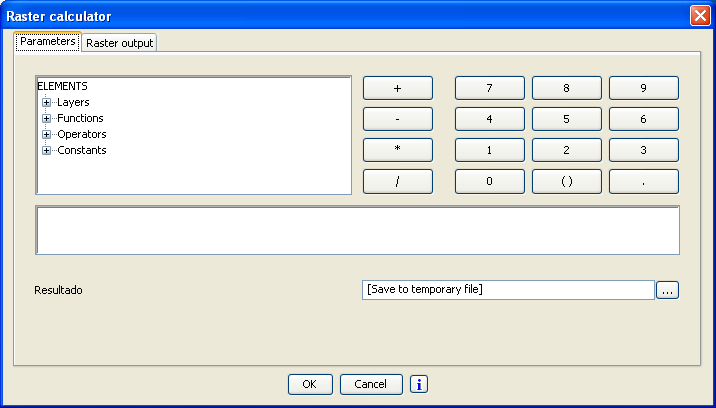
\includegraphics[width=.7\textwidth]{gridCalculator.png} 
\end{center}

Clearly, this is not the typical parameters panel. You can see the \emph{Raster output} tab, but the parameters panel is different and it has a more elaborated design. SEXTANTE features a flexible mechanism that allows developers to create their own interfaces in case the default one does not meet their needs. 

Let's suppose we want an user interface for our algorithm, which is implemented in the \texttt{MultiplyRasterAlgorithm} class. Here is what you have to do to create an user interface tailored to the needs of your algorithm.

\begin{itemize}
	\item Add a new class named \emph{MultiplyRasterParametersPanel} to the same package the algorithm class belongs to. That is, the name of the algorithm, but replacing the suffix \texttt{Algorithm} by the prefix \texttt{ParametersPanel}. 
	\item This class has to extend the \texttt{GeoAlgorithmParametersPanel} class, which extends the \texttt{JPanel} class. When SEXTANTE creates the algorithm dialog, it will add the parameters tab and the raster output tab if needed. It will look for a class with the same name as the algorithm but with the suffix \texttt{ParametersPanel}. If such a class exists and it extends the \texttt{GeoAlgorithmParametersPanel} class, it will add the panel represented by that class to the parameters tab. If not, it will generate a default panel based on the characteristics of the algorithm.
	\item Create your UI. If you need a list of layers or tables to show it to the user, the current input factory can help you do that. For instance, to get a list of raster layers, you can do the following.
	
	\begin{verbatim}
	IRasterLayer[] layers = SextanteGUI.getInputFactory().getRasterLayers();
	\end{verbatim}
	
	Your class must have a constructor with no arguments and you have to override the \texttt{init(GeoAlgorithm)} method, which should itself create the GUI. This method will be called by SEXTANTE just after instantiating the class.
	\item There is another method that you have to override from the \texttt{GeoAlgorithmParametersPanel} class. It is named \emph{boolean assignParameters()} and you have to add there all the code needed to assign the values entered or selected by the user in your GUI to the corresponding parameters of the algorithm. You should check the validity of those values in this method, and return true if they are correct, or false otherwise.
\end{itemize}

	
\subsection{Customizing the interface for the modeller}
	
{\bfseries[section yet to be written]}

\section{More examples}

Want more examples? SEXTANTE contains more than 250 algorithms, all of them implemented following the ideas described in this chapter. They are a great source of information, and having a look at their source code will for sure help you to better understand all the concepts and techniques we have already seen.

If you are looking for simple and easy--to-understand algorithms, have a look at the \emph{gridTools} and \emph{vectorTools} projects. They are a good point to start.

